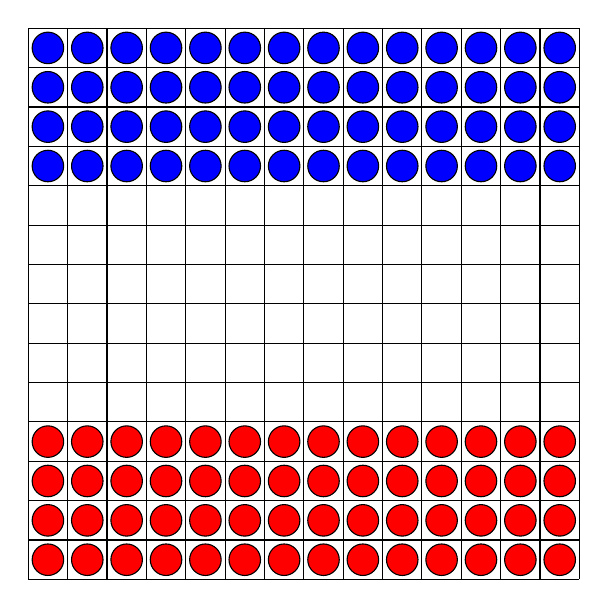
\begin{tikzpicture}[scale=0.5]
	% Cols
	\foreach \i in {0, ..., 14} {
		\draw [thin, black] (\i,0) -- (\i,14);
	}
	% Rows
	\foreach \i in {0, ..., 14} {
		\draw [thin, black] (0,\i) -- (14,\i);
	}
	% Red
	\foreach \r in {1, ..., 4} {
		\foreach \l in {1, ..., 14} {
			\draw [color=black, fill=red] (\l-0.5,\r-0.5) circle (0.4); 		
		}
	}
	% Blue
	\foreach \r in {11, ..., 14} {
		\foreach \l in {1, ..., 14} {
			\draw [color=black, fill=blue] (\l-0.5,\r-0.5) circle (0.4); 		
		}
	}
\end{tikzpicture}